\documentclass[letterpaper,9pt,twocolumn,twoside,]{pinp}

%% Some pieces required from the pandoc template
\providecommand{\tightlist}{%
  \setlength{\itemsep}{0pt}\setlength{\parskip}{0pt}}

% Use the lineno option to display guide line numbers if required.
% Note that the use of elements such as single-column equations
% may affect the guide line number alignment.

\usepackage[T1]{fontenc}
\usepackage[utf8]{inputenc}

% pinp change: the geometry package layout settings need to be set here, not in pinp.cls
\geometry{layoutsize={0.95588\paperwidth,0.98864\paperheight},%
  layouthoffset=0.02206\paperwidth, layoutvoffset=0.00568\paperheight}

\definecolor{pinpblue}{HTML}{185FAF}  % imagecolorpicker on blue for new R logo
\definecolor{pnasbluetext}{RGB}{101,0,0} %



\title{Variación de la altura de Vismia Macrophylla y Jacaranda Copaia a través
de diferentes estados de sucesión de un bosque húmedo tropical de
acuerdo con sus hábitos de crecimiento}

\author[a]{Camilo Cruz Sanchez}
\author[a]{Yonatan Moran Ruano}
\author[a]{Elkin Vanegas Vargas}
\author[a]{Cristian Gañan Tapasco}

  \affil[a]{Departamento de ciencias forestales, Univeridad Nacional de Colombia,
Medellín}

\setcounter{secnumdepth}{0}

% Please give the surname of the lead author for the running footer
\leadauthor{Sanchez-Moran-Vanegas-Gañan}

% Keywords are not mandatory, but authors are strongly encouraged to provide them. If provided, please include two to five keywords, separated by the pipe symbol, e.g:
 \keywords{  one |  two |  optional |  keywords |  here  }  

\begin{abstract}
Your abstract will be typeset here, and used by default a visually
distinctive font. An abstract should explain to the general reader the
major contributions of the article.
\end{abstract}

\dates{This version was compiled on \today} 

% initially we use doi so keep for backwards compatibility
% new name is doi_footer
\doifooter{Depertamento de ciencias forestales}

\pinpfootercontents{Ecología Forestal}

\begin{document}

% Optional adjustment to line up main text (after abstract) of first page with line numbers, when using both lineno and twocolumn options.
% You should only change this length when you've finalised the article contents.
\verticaladjustment{-2pt}

\maketitle
\thispagestyle{firststyle}
\ifthenelse{\boolean{shortarticle}}{\ifthenelse{\boolean{singlecolumn}}{\abscontentformatted}{\abscontent}}{}

% If your first paragraph (i.e. with the \dropcap) contains a list environment (quote, quotation, theorem, definition, enumerate, itemize...), the line after the list may have some extra indentation. If this is the case, add \parshape=0 to the end of the list environment.


\hypertarget{introduccuxedon}{%
\section{Introduccíon}\label{introduccuxedon}}

Colombia presenta una alta diversidad biológica, amenazada por la
intensa presión antrópica que envuelve la deforestación, la
fragmentación y los cambios en el uso del suelo, causados principalmente
por actividades ganaderas y agrícolas.\citep{salas} Las áreas que se
recuperan de la perturbación, donde se ha practicado principalmente la
agricultura de subsistencia de roza y quema, y zonas de pastura para la
ganadería, generan un aumento de los bosques secundarios\citep{hammer}
que han venido presentando una regeneración a través del tiempo.

La Regeneración del ecosistema hace parte de un proceso dinámico en el
cual nuevos individuos entran a hacer parte de la población reproductora
a medida de que otros mueren por medio de un proceso natural
/citep\{pulido\}, dando así paso a nuevas especies más prósperas en las
condiciones que surgen a partir del cambio de vegetación y variables
climáticas. La incidencia de las prácticas forestales o agrícolas suele
alterar los parámetros de regeneración del bosque ya que esto altera
condiciones esenciales para la vida de ciertas especies cambiando así la
evolución natural del bosque \citep{pulido}.

Para el estudio de la regeneración o sucesión ecológica en el bosque
húmedo tropical de la La Reserva Natural Hacienda San Pedro ubicada en
la cuenca media del río Magdalena se definen cuatro estados sucesionales
de crecimiento del bosque: SS1: sucesión en edad de 0-5 años, con área
de 30 ha, presencia de pastos, escasa vegetación arbórea y donde
predominó la actividad ganadera; SS2: sucesión en edad de 10-13 años con
vegetación arbórea, con área de 50 ha, con presencia de helechos y
dominio de especies heliófilas de rápido crecimiento, con suelo
anteriormente usado en actividades agrícolas; SS3: sucesión con edad de
18-20 años, con área de 40ha, con algunos árboles de altura mayor a 30m
y un dosel más cubierto, con presencia de epífitas y especies tolerantes
a la sombra y con suelo antes usado en actividades ganaderas; SS4:
sucesión avanzada con edad mayor a 50 años, con área de 180 ha, con
grandes árboles y dosel cubierto, con pocos claros y presencia de
epífitas y bromelias y con presencia de bosque anteriormente sometido a
tala selectiva.

En esta reserva se realizó un levantamiento de datos por medio de 4
parcelas ubicadas según las condiciones topográficas y logísticas, donde
se tuvieron en cuenta dos especies, la primera \emph{Jacaranda Copaia}
que es un árbol grande de hasta 35 m de altura que vive mejor a una
altura de 0 a 1000 msnm, siendo este de tipo heliófita y una especie
pionera en la regeneración de bosques \citep{tapia}, la cual se
encontraron muy pocos individuos en todas las parcelas y la segunda,
\emph{Vismia Macrophylla}, árbol o arbusto característico de lugares en
barbecho, enrastrojados o áreas de pastos cercanas a bosques
fragmentados, de tipo Heliófita \citep{leza}, puede llegar a medir hasta
12 m de altura, presente más comúnmente entre los 10 a 700
msnm\citep{vismia}. Con dichas especies se realizó una comparación entre
los estados sucesionales de crecimiento y el cambio en la altura de
estas dos especies en las diferentes parcelas por medio de los modelos
Weibull y Michaelis Menten.

Las radiación que llega a un determinado lugar influyen en numerosos
procesos fisiológicos, reproductivos de plantas, y afecta de forma muy
significativa el funcionamiento general del ecosistema. Los rasgos de la
radiación que tienen relevancia ecológica y evolutiva son: la
intensidad, la calidad, la direccionalidad, y la distribución en el
tiempo y en el espacio. Además, la luz es el factor abiótico más
variable en el tiempo y en el espacio, el análisis de esta variabilidad,
así como sus causas y consecuencias , supone una de las mejores
aproximaciones al estudio de la luz como un factor ecológico y evolutivo
muy importante. \citep{vallares} Es por eso que mediante un análisis de
porcentaje de radiación que pasa a través del dosel realizado con el
software ImageJ por medio de fotos tomadas en medio del dosel dentro de
las parcelas, se espera que muestre la disminución en la disponibilidad
de luz a medida que la regeneración del bosque es más avanzada y con
esto analizar el comportamiento en la cantidad de individuos encontrados
en cada parcela de las especies mencionadas anteriormente según sus
hábitos de crecimiento y el gremio ecológico que presentan.

Con todo esto se espera responder cómo varía la altura de Vismia
Macrophylla y Jacaranda Copaia a través de los diferentes estados de
sucesión de un bosque húmedo tropical de acuerdo con sus hábitos de
crecimiento.

\hypertarget{materiales-y-muxe9todos}{%
\section{Materiales y métodos}\label{materiales-y-muxe9todos}}

\hypertarget{localizaciuxf3n-y-descripciuxf3n-del-uxe1rea-de-estudio}{%
\subsection{Localización y descripción del área de
estudio}\label{localizaciuxf3n-y-descripciuxf3n-del-uxe1rea-de-estudio}}

La Reserva Natural Hacienda San Pedro tiene carácter privado, con una
extensión total de \(300ha\) y predominio de áreas con bosque secundario
en regeneración natural. Se encuentra ubicada en la cuenca media del río
Magdalena, junto al río Nus
\((6^{\circ} 27'35'' N\ , \ 74^{\circ} 47'15'' W)\), en el Municipio
Maceo, Departamento de Antioquia, Colombia \textbf{Fig.1}. Tiene una
temperatura media de \(23,8^{\circ}C\), una humedad relativa del
\(87\%\) y una precipitación media anual de \(2.757mm\), para la
estación meteorológica Caracolí (\(2308053\) - Red Hidrometeorológica de
Empresas Públicas de Medellín \(–EE.PP.M-\)). Se encuentra en zona de
Bosque Húmedo Premontano \((bh-P)\) y Bosque Húmedo Tropical \((bh-T)\),
en un rango altitudinal de \(800\) a \(1.100m\) \(s.n.m\).

\begin{figure}[h]
  \centering
  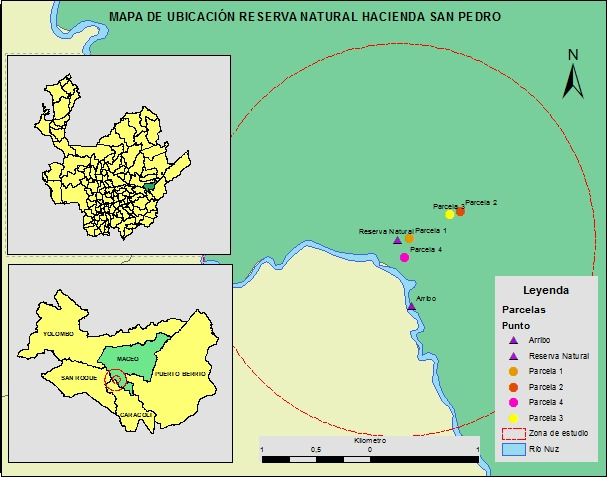
\includegraphics[width= 0.5\textwidth]{figure1.jpeg}
  \caption{Reserva Natural Hacienda San Pedro}
\end{figure}

El desarrollo del presente trabajo se dio en dos etapas las cuales se
describen a continuación:

\hypertarget{levantamiento-de-informaciuxf3n}{%
\subsubsection{1) Levantamiento de
información}\label{levantamiento-de-informaciuxf3n}}

Para la recolección de la información se procedió a establecer áreas
determinadas para cada parcela estudiada de acuerdo con condiciones como
la topografía y logísticas que permitieran el desarrollo del trabajo. Se
centró la recolección de la información en especies de plantas comunes
en las diferentes parcelas; para el caso del presente análisis se
trabajaron las especies Vismia Macrophylla y Jacaranda Copaia. Las áreas
de las parcelas y especificaciones se se relacionan en la \textbf{Table
1}:

\begin{table}

\caption{\label{tab:unnamed-chunk-1}Areas de parcelas trabajadas}
\centering
\begin{tabular}[t]{r|r|l|l|l}
\hline
Parcela & Área (m2) & Figura geométrica & Dimensiones (m) & Sucesión\\
\hline
1 & 500 & Circunferencia & r = 12,62 & SS1\\
\hline
2 & 324 & Cuadrado & 18 x 18 & SS3\\
\hline
3 & 450 & Rectángulo & 30 x 15 & SS2\\
\hline
4 & 800 & Rectángulo & 40 x 20 & SS1\\
\hline
\end{tabular}
\end{table}

Una vez establecidas las parcelas se procedió a recolectar la
información de las correspondientes especies, para la recolección de
esta información se procedió a categorizar las especies en tres tamaños
los cuales fueron Brinzales, Latizales y Fustales; dicha descripción se
presenta en la \textbf{Table 2}

\begin{table}

\caption{\label{tab:unnamed-chunk-2}Catregorias de especies}
\centering
\begin{tabular}[t]{l|l|l}
\hline
Categoría vegetación & Tamaño DAP (cm) & Altura (m)\\
\hline
Brinzales & <5 & 1 - 1,5\\
\hline
Latizales & 5-10 & NA\\
\hline
Fustales & >10 & NA\\
\hline
\end{tabular}
\end{table}

Posterior al montaje de cada una de las parcelas se procedió a medir la
altura \((m)\) y \(DAP \ (cm)\) de las especies que se estudiaron. Para
el registro de los datos se utilizó la \texttt{App\ Memento} en la cual
se tuvo en cuenta la corrección por pendiente para el caso de la
categoría de fustales, para el caso de los latizales no se hizo
corrección por pendiente y en el caso de los brinzales se realizó la
respectiva medición con la cinta métrica. En cada una de las parcelas se
observaron características bióticas y abióticas como lo fueron
vegetación dominante, cobertura, características sustrato, topografía y
perturbaciones (antrópicas o naturales).

Otro de los aspectos que se tomó en cuenta en la recolección de los
datos fueron las fotografías bajo el dosel de cada una de las parcelas
con el objetivo de realizar la respectiva caracterización de radiación
que pasa a través del dosel y entender la relación que tiene con el
estado de sucesión de las parcelas, también se tomaron dichas
fotografías para observar la relación que guarda la radiación con los
hábitos de crecimiento de las especies que se analizaron.

\hypertarget{procesamiento-de-los-datos-recolectados}{%
\subsubsection{2) Procesamiento de los datos
recolectados}\label{procesamiento-de-los-datos-recolectados}}

\hypertarget{a-ajuste-del-modelo}{%
\paragraph{a) Ajuste del modelo}\label{a-ajuste-del-modelo}}

Se ajustó un modelo que describiera la altura en función del \(DAP\). El
modelo biológicamente correcto presenta comúnmente una forma sigmoidea
con un punto de inflexión en la parte inferior de los datos o bien forma
cóncava sin punto de inflexión aparente \citep{huan}, esto sugiere
modelos no lineales que ajusten el comportamiento esperado; por
experiencia se sabe que hay modelos alométricos que describen lo ya
mencionado, es el caso del modelo Weibull y Michaelis Menten, estos se
escogieron para el ajuste, pues son funciones que siguen la ontogenia
natural. Para hacerlos, se tuvo que ordenar los datos, algunos de estos
no eran lógicos, se encontró DAP del orden de \(2cm\) o menos con
alturas de \(96 m\) lo cual no es posible, se halló que todos los datos
no superan \(50 m\) de altura, excepto algunos con el problema descrito,
se hace un filtro de Altura \(< \ 50 m\), con esto, se ajustan los
modelos para las dos especies en cuestión.

\hypertarget{b-procesamiento-de-fotografuxedas-del-dosel}{%
\paragraph{b) Procesamiento de fotografías del
dosel}\label{b-procesamiento-de-fotografuxedas-del-dosel}}

El dosel influye en la cantidad de radiación del bosque dependiendo de
la cantidad de radiación directa o indirecta que llegue al ecosistema.
la penetración de la radiación depende de la localización, del tamaño,
la arquitectura y altura del dosel. la radiación lumínica disponible se
estimó mediante fotografías realizadas en campo. las imágenes se
procesaron con el software \texttt{imagenJ}. Este programa convierte las
fotos en imágenes binarias de blancos y negros (Fig.2). De esta manera
se puede obtener el porcentaje blancos en cada fotografía, asumiendo
este como el porcentaje de radiación que atraviesa el dosel como se
puede observar en la tabla 3 .

\begin{figure}[h]
  \centering
  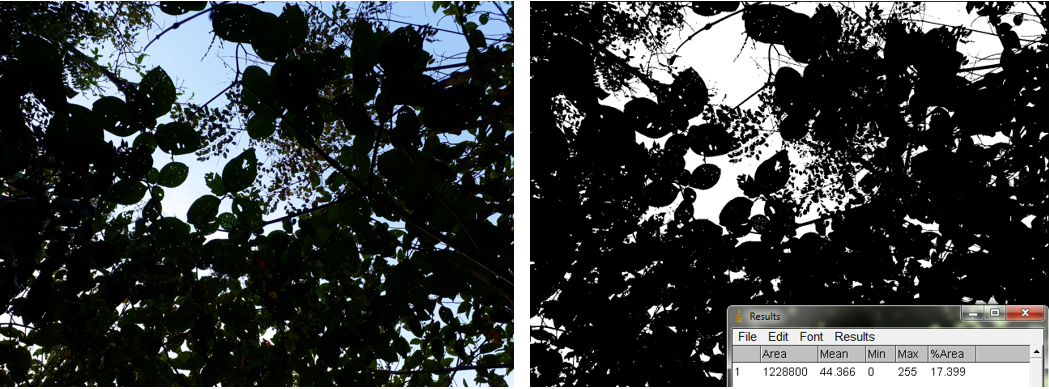
\includegraphics[width= 0.5\textwidth]{ima2.png}
  \caption{Conversión de imagenes a blancos y negros}
\end{figure}

\hypertarget{resultados}{%
\section{Resultados}\label{resultados}}

La forma y la disposición del dosel en las diferentes parcelas y sus
respectivos estados de sucesión dieron lugar a dos grupos de formaciones
significativas sobre la radiación disponible en el bosque. El primero de
ellos comprende las parcelas 1,3 y 4 que pertenecen a los estados de
sucesión SS1, SS2 Y SS1 respectivamente donde en las parcelas 1 y 4 se
puede encontrar presencia de pastos y escasa vegetación arbórea, en la
parcela 3 cuenta con vegetación arbórea, con presencia de helechos y
especies heliófilas de rápido crecimiento. Es por eso que este primer
grupo la radiación en el bosque fue en promedio de un \(17 \%\)
(\textbf{Table 3}) de radiación disponible. Por otro lado la parcela 2
perteneciente al estado de sucesión SS3 donde la radiación disponible no
superó el \(8 \%\) (\textbf{Table 3}) debido a que en este estado
teniendo en cuenta su edad de regeneración se puede encontrar algunos
árboles de altura mayor de \(30 m\) y de esta manera teniendo un dosel
más cubierto, permitiendo un menor ingreso de radiación al interior del
bosque, esta ausencia de radiación disponible explica la presencia de
plantas epifitas y especies tolerantes a la sombra.

\begin{table}

\caption{\label{tab:unnamed-chunk-3}Porcentaje de radiación que atraviesa el dosel}
\centering
\begin{tabular}[t]{r|l|l|l}
\hline
Parcela & Sucesión & \%R que atraviesa dosel & \%R que No atraviesa dosel\\
\hline
1 & SS1 & 17.4 & 82.6\\
\hline
2 & SS3 & 8.92 & 91, 08\\
\hline
3 & SS2 & 17, 15 & 82, 85\\
\hline
4 & SS1 & 17, 38 & 82, 62\\
\hline
\end{tabular}
\end{table}

\hypertarget{modelo-michaelis-menten}{%
\section{Modelo Michaelis Menten}\label{modelo-michaelis-menten}}

El modelo Weibull a pesar de tener un RSE de 2.67 con un AIC de 873.76
frente al Michaelis Menten RSE de 2.70 con un AIC de 876.90, no se puede
escoger como el mejor modelo pues gráficamente tiende disminuir la
altura a medida que aumenta el DAP \textgreater{} 25 lo cual no tiene
sentido, lo normal sería un tendencia asintótica a medida que aumenta el
DAP; por esta razón se elige al modelo de Michaelis Menten como el
modelo que ajusta mejor a los datos, pues sigue la tendencia natural.

\begin{figure}

{\centering 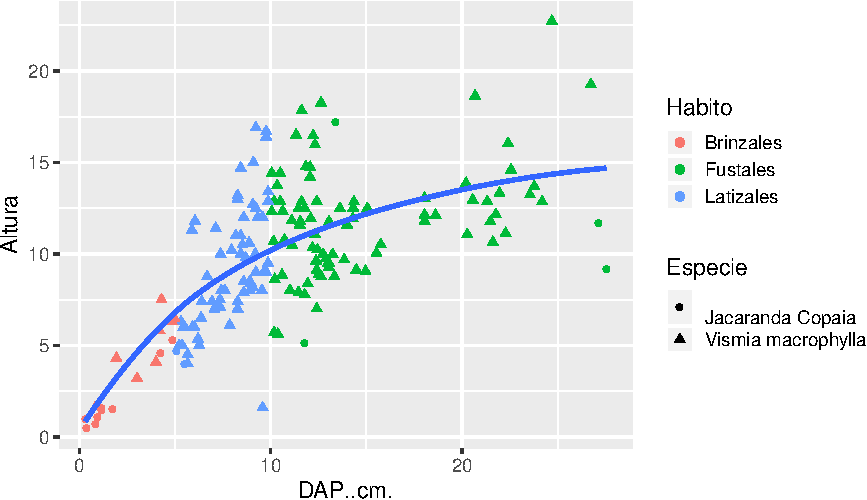
\includegraphics{report_ecology_files/figure-latex/unnamed-chunk-6-1} 

}

\caption{Modelo Michaelis Menten parcela-especie}\label{fig:unnamed-chunk-6}
\end{figure}

\begin{figure}

{\centering 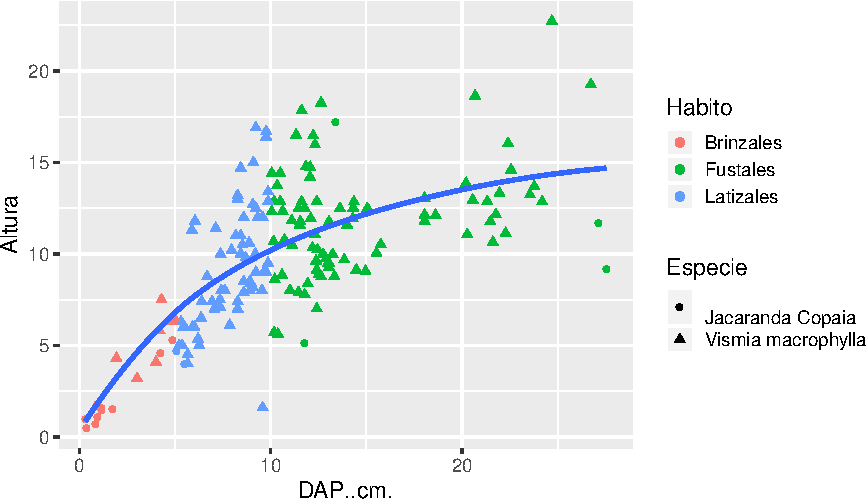
\includegraphics{report_ecology_files/figure-latex/unnamed-chunk-7-1} 

}

\caption{Modelo Michaelis Menten especie-habito}\label{fig:unnamed-chunk-7}
\end{figure}

\begin{table}

\caption{\label{tab:unnamed-chunk-8}Diametro cuadratico medio}
\centering
\begin{tabular}[t]{l|r}
\hline
Habito & Dcm\\
\hline
Brinzales & 3.145550\\
\hline
Fustales & 15.675398\\
\hline
Latizales & 8.074326\\
\hline
\end{tabular}
\end{table}

\begin{figure}

{\centering 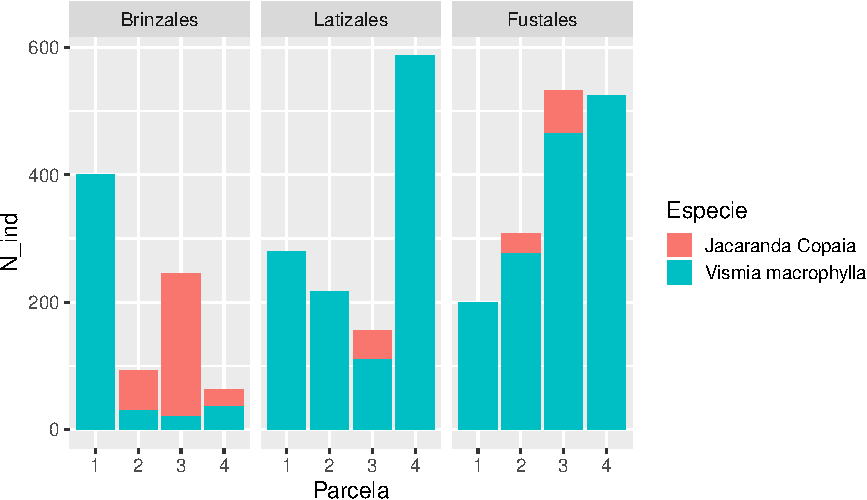
\includegraphics{report_ecology_files/figure-latex/unnamed-chunk-10-1} 

}

\caption{Número de individuos por parcela}\label{fig:unnamed-chunk-10}
\end{figure}

\begin{table}

\caption{\label{tab:unnamed-chunk-11}Numero de individuos por hectarea}
\centering
\begin{tabular}[t]{l|l|r|l}
\hline
Parcela & Habito & N\_ind & Especie\\
\hline
2 & Brinzales & 61.72840 & Jacaranda Copaia\\
\hline
2 & Fustales & 30.86420 & Jacaranda Copaia\\
\hline
3 & Brinzales & 222.22222 & Jacaranda Copaia\\
\hline
3 & Fustales & 66.66667 & Jacaranda Copaia\\
\hline
3 & Latizales & 44.44444 & Jacaranda Copaia\\
\hline
4 & Brinzales & 25.00000 & Jacaranda Copaia\\
\hline
1 & Brinzales & 400.00000 & Vismia macrophylla\\
\hline
1 & Fustales & 200.00000 & Vismia macrophylla\\
\hline
1 & Latizales & 280.00000 & Vismia macrophylla\\
\hline
2 & Brinzales & 30.86420 & Vismia macrophylla\\
\hline
2 & Fustales & 277.77778 & Vismia macrophylla\\
\hline
2 & Latizales & 216.04938 & Vismia macrophylla\\
\hline
3 & Brinzales & 22.22222 & Vismia macrophylla\\
\hline
3 & Fustales & 466.66667 & Vismia macrophylla\\
\hline
3 & Latizales & 111.11111 & Vismia macrophylla\\
\hline
4 & Brinzales & 37.50000 & Vismia macrophylla\\
\hline
4 & Fustales & 525.00000 & Vismia macrophylla\\
\hline
4 & Latizales & 587.50000 & Vismia macrophylla\\
\hline
\end{tabular}
\end{table}

%\showmatmethods


\bibliography{pinp}
\bibliographystyle{jss}



\end{document}

